\section{Ziel}
In diesem Versuch wird eine Hochvakuumdiode untersucht, um  die Austrittsarbeit der Elektronen bei Wolfram zu bestimmen.
Hierzu werden verschiedene Kennlinien gemessen und der Gültigkeitsbereich des Langmuir-Schottkyschen Raumladungsgesetzes gesucht.
Außerdem wird das Anlaufstromgebiet der Diode untersucht.






\section[Theorie]{Theorie\footnote[1]{Unter Verwendung von \cite{man:v504}.}}

% \subsection{Einleitung}
Grundlage dieses Versuchs ist der glühelektrische Effekt, bei dem durch Erwärmung von Metalloberflächen Elektronen emittiert werden können.
Dabei ist insbesondere die Austrittsarbeit als Materialkonstante von Interesse.
Hierfür ist eine Hochvakuumdiode nötig, damit die Elektronen nicht mit der Luft wechselwirken.



\subsection{Austrittsarbeit und Energieverteilung von Leitungselektronen}
In Metallen sind ionisierte Atome auf einer Kristallgitterstruktur angeordnet.
Die Atome sind dabei von freigesetzten Elektronen eingehüllt, die nicht mehr einem bestimmten Atom zugeordnert werden können.
Daher werden sie auch Leitungselektronen genannt.
In grober Näherung kann für das Gitterpotential das Potentialtopfmodell verwendet werden.
Im Inneren des Metalls gibt es dabei ein positives konstantes Potential, welches allerdings um den Betrag $\xi$ geringer ist als im Außenraum des Metalls, vgl. Abbilung \ref{fig:potentialtopf_metall}.
Auf die Leitungselektronen wirken folglich keine Kräfte und sie können sich frei bewegen.
Deshalb haben Metalle eine sehr gute elektrische Leitfähigkeit.
Zum Verlassen des Metalls muss ein Elektron somit die Austrittsarbeit
\begin{align}
    W = e_0 \xi % \text{e}_0 \xi
    \label{eq:austrittsarbeit}
\end{align}
aufwenden.

\begin{figure}[H]
    \centering
    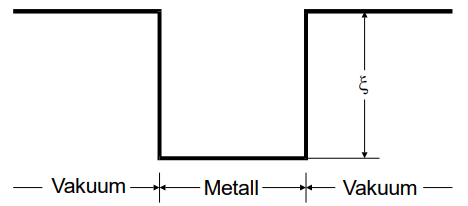
\includegraphics[height = 3 cm]{Abbildungen/potentialtopf_metall.png}
    \caption{Der Potentialtopf eines Metalls \cite[]{man:v504}.}
    \label{fig:potentialtopf_metall}
\end{figure}


\noindent
Um zu überprüfen, ob die innere Energie der Elektronen zum spontanen Verlassen der Oberfläche ausreicht, muss die Quantentheorie betrachtet werden.
Zum einen können die Elektronen nur diskrete Energiewerte annnehmen.
Zum anderen kann ein Zustand mit Energie $E$ aufgrund des Pauli-Verbots von maximal 2 Elektronen mit entgegengesetztem Spin besetzt werden.
Dadurch haben die Elektronen selbst für $T = 0$ eine endliche Energie. 
Die sogenannte Fermische Grenzenergie $\zeta$ ist die Maximalenergie der Elektronen bei $T = 0$.
Bei Zimmertemperatur gilt $\zeta >> k_\text{B} T$.
Die Fermi-Diracsche Verteilungsfuktion 
\begin{align}
    f(E) = \frac{1}{\exp\left(\frac{\zeta - E}{k_\text{B} T}\right) + 1}
    \label{eq:fermi_dirac}
\end{align}
beschreibt die Wahrscheinlichkeit, dass im thermischen Gleichgewicht ein möglicher Zustand mit der Energie $E$ besetzt ist.
Dadurch, dass selbst beim Schmelzpunkt von Wolfram $E$ groß gegen $k_\text{B} T$ ist, kann die Funktion durch
\begin{align}
    f(E) = \exp\left(\frac{\zeta - E}{k_\text{B} T}\right)
    \label{eq:energieverteilung}
\end{align}
genähert werden.




\subsection{Die Sättigungsstromdichte}
Von Interesse ist die Sättigungsstromdichte $j_\text{s}(T)$, d.h. die temperaturabhängige Elektronenanzahl, die pro Zeit- und Flächeneinheit aus der Oberfläche 
des Metalls austreten.
% Hierfür wird das Koordinatensystem so gelegt, dass die $z$-Achse senkrecht auf der ebenen Oberfläche steht.
Es lässt sich mit einigen Überlegungen (vgl. \cite{man:v504}) die Richardson-Gleichung
\begin{align}
    j_\text{s}(T) = \frac{4 \pi}{h^3} e_0 m_0 k_\text{B}^2 T^2 \exp\left(- \frac{\text{e}_0 \xi}{k_\text{B} T}\right)
    \label{eq:richardson}
\end{align}
herleiten, wobei $m_0$ die Elektronenmasse ist.
Diese lässt sich zur Austrittsarbeit 
\begin{align}
    W = e_0 \xi = - k_\text{B} T \cdot \ln\left(\frac{h^3 j_\text{S}}{4 \pi e_0 m_0 k_\text{B}^2 T^2}\right)
    \label{eq:austritt_richardson}
\end{align}



\subsection{Hochvakuumdiode}
Der Sättigungsstrom kann nur im Hochvakuum gemessen werden, da die Elektronen ansonsten mit den Gasmolekülen wechselwirken würden.
Ferner wird ein elektrisches Feld zum Absaugen der Elektronen nötig.
Beide Eigenschaften werden in einer Hochvakuumdiode realisiert, die scheamtisch in Abbilung \ref{fig:hochvakuumdiode} zu sehen.
In einem evakuierten Glaskörper ist eine Glühkathode eingeschlossen, 
die durch einen angelegten Gleichstrom auf $\qtyrange[]{1000}{3000}{\kelvin}$ errhitzt werden kann.
Das elektrisches Feld wird durch eine Saugspannung zwischen der Kathode und der gegenüberliegenden Anode erzeugt.
Es wird hier von einer Diode gesprochen, da nur dann ein Strom fließen kann, wenn die Anode positiv gegenüber der Kathode ist.
Es sei angemerkt, dass die Emission der Anode wegen ihrer niedrigen Temperaturen viele Größenordnungen niedriger als die der Kathode ist.

\begin{figure}[H]
    \centering
    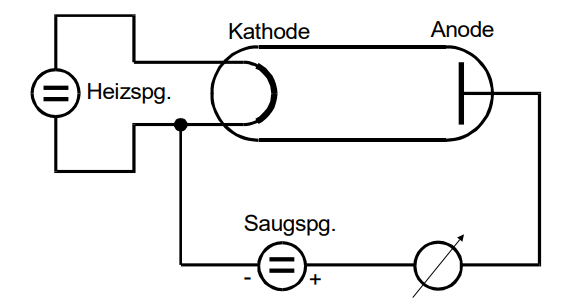
\includegraphics[height = 4cm]{Abbildungen/hochvakuum_diode.png}
    \caption[]{Schematische Darstellung der Hochvakuumdiode \cite{man:v504}.}
    \label{fig:hochvakuumdiode}
\end{figure}



\subsection{Langmuir-Schottkysche Raumladungsgleichung}
Der Anodenstrom hängt bei gegebener Kathodentemperatur auch von der Anodenspannung $U_\text{A}$ ab.
Wird $U_\text{A}$ zu niedrig gewählt, erreichen nicht alle Elektronen die Anode.
Damit der Strom einen Sättigungswert $I_\text{S}$ erreicht und unabhängig von $U_\text{A}$ ist, 
muss $U_\text{A}$ hinreichend groß gewählt werden.
Dennoch gilt das Ohmsche Gesetz auch vor erreichen von $I_\text{S}$ nicht, da die Elektronen zur Anode hin beschleunigt werden.
Dadurch hängt die Raumladung $\rho$ vom Ort ab. 
In der Nähe der Anode ist $\rho$ kleiner als in der Nähe der Kathode.
Dies folgt aus der Kontinuitätsbedingung $j = \rho v = \text{const}$, wobei $v$ die Geschwindigkeit ist.
In anderen Worten bedeutet das, dass $\rho$ das elektrische Feld der Anode von der Kathode abschirmt und nicht alle Elektronen die Anode erreichen.
Folglich ist der Anodenstrom kleiner als der nach Gleichung \eqref{eq:richardson} erwartete Strom.
Der Zusammenhang zwischen Anodenspannung $U_\text{A}$ und -stromdichte $j_\text{A}$ im Raumladungsbereich kann mit einigen Zwischenschritten
(vgl. \cite{man:v504}) zum Langmuir-Schottkyschen Raumladungsgesetz
\begin{align}
    j_\text{A}\left(U_\text{A}\right) = \frac{4}{9 a^2} \epsilon_0 \sqrt[]{2 \frac{e_0}{m_0} U_\text{A}^3}
    \label{eq:lang_schott}
\end{align}
bestimmt werden, d.h. es gibt eine Proportionalität von $j \propto U_\text{A}^\frac{3}{2}$.
Dabei ist $a$ der Abstand zwischen Anode und Kathode.
Der Gültigkeitsbereich dieses Gesetzes wird Raumladungsgebiet genannt.





\subsection{Anlaufstromgebiet}
Dem Langmuir-Schottkyschen Gesetz \eqref{eq:lang_schott} ist zu entnehmen, dass für eine Spannung von $U_\text{A} = \qty[]{0}{\volt}$ kein Strom gemessen werden kann.
Da die Elektronen allerdings eine Geschwindigkeit beim Verlassen der Kathode aufweisen, ist dennoch ein Strom messbar.
Der Fermi-Dirac-Verteilung \eqref{eq:fermi_dirac} ist zu entnehmen, dass es endlich viele Elektronen mit einer Energie gibt, 
die größer als die Austrittsarbeit ist.
Die überschüssige Energie nach Verlassen des Metalls geht in die kinetische Energie der Elektronen über.
Folglich sind die Elektronen in der Lage, gegen ein Gegenfeld anzulaufen, weshalb der resultierende Storm auch Anlaufstrom genannt wird.

\noindent
Die Energieverhältnisse im Anlaufstromgebiet ($U_\text{A} = V < 0$) sind in Abbildung \ref{fig:potential_anlaufstrom} zu sehen.
Dabei ist $e_0 \phi_\text{A}$ die Austrittsarbeit der Anode und $e_0 \phi_\text{K}$ die Austrittsarbeit der Kathode.
Der Abbildung ist entnehmbar, dass Elektronen mit einer Energie $E \geq e_0 (\phi_\text{A} + U_\text{A})$ die Anode erreichen.
Gemäß der Energieverteilung \eqref{eq:energieverteilung} der Elektronen kann der Zusammenhang im Anlaufstromgebiet expontentiell durch
\begin{align}
    j(U_\text{A}) = b \cdot \exp\left(-\frac{e_0 U_\text{A}}{k_\text{B} T}\right)
\end{align}
mit einer Konstante $b$ gefolgert werden.

\begin{figure}[H]
    \centering
    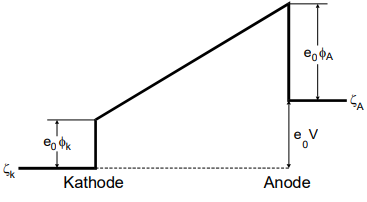
\includegraphics[height = 4 cm]{Abbildungen/potential_anlaufstrom.png}
    \caption{Potenitalverhältnisse im Anlaufstrombereich \cite[]{man:v504}.}
    \label{fig:potential_anlaufstrom}
\end{figure}



\subsection{Kennlinien der Hochvakuumdiode}
Die Kennlinie einer hochvakuumdiode ist der Zusammenhang zwischen Anodenstrom $I_\text{A}$ bzw. -dichte $j_\text{A}$ und der angelegten
Anodenspannung $U_\text{A}$, wobei es insgesamt drei Bereiche gibt.
Als erstes gibt es einen expontentiellen Zusammenhang zwischen den Messgrößen für $U_\text{A} < 0$ beim Anlaufstrom.
Danach folgt eine Abhängigkeit von $I_\text{A} \propto \sqrt{U_\text{A}^3}$ bei der Raumladungsdichte $\rho$.
Da diese allerdings unabhängig von der Anodenspannung $U_\text{A}$ ist, kann diese Abhängigkeit nicht für alle $U_\text{A}$ gelten.
Somit tritt irgendwann Sättigung ein (vgl. Gleichung \eqref{eq:richardson}). 
Fügt man die drei Bereiche des Anlaufstroms, der Raumladungsdichte und der Sättigung zusammen, ergibt sich ein Bild 
wie in Abbildung \ref{fig:kennlinie} bei fester Temperatur $T$.

\begin{figure}[H]
    \centering
    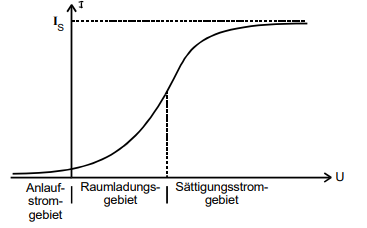
\includegraphics[height = 5 cm]{Abbildungen/kennlinie.png}
    \caption{Die Kennlinie einer Hochvakuumdiode \cite[]{man:v504}.}
    \label{fig:kennlinie}
\end{figure}






\subsection{Kathodentemperatur}
Zur Bestimmung der Kathodentemperatur $T$ kann die Leistungsbilanz betrachtet werden.
Die der Kathode zugeführte Leistung $N_\text{zu} = U_\text{Heiz} I_\text{Heiz}$ mit Heizspannung und -strom $U_\text{Heiz}$ bzw. 
$I_\text{Heiz}$ setzt sich aus der Strahlungsleistung $N_\text{Str}$ und der Wärmeleitung $N_\text{Leit}$ zusammen.
Dabei gilt für die Strahlungsleistung das Stefan-Boltzmann-Gesetz
\begin{align}
    N_\text{Str} = F \eta \sigma T^4
\end{align}
mit der emittierenden Kathodenoberfläche $F = \qty{0.32}{\cm}^2$, dem Emissionsgrad $\eta = \num{0.28}$ und der 
Boltzmannschen Strahlungskonstante $\sigma = \num[]{5.7} \cdot 10^{-12} \, \frac{\unit{\watt}}{\unit{\cm}^2\unit{\kelvin}^4}$.
Ferner kann für die vorhandene Apparatur $N_\text{Leit} = \qtyrange{0.9}{1}{\watt}$ geschätzt werden.
Insgesamt ergibt sich 
\begin{align}
    N_\text{zu} = U_\text{Heiz} I_\text{Heiz} = N_\text{Str} + N_\text{Leit} = F \eta \sigma T^4 + N_\text{Leit}.
    \label{eq:leistung}
\end{align}
